\documentclass{article}
\usepackage{graphicx}
\usepackage[polish]{babel}
%\usepackage{polski}
\usepackage[utf8]{inputenc}
\usepackage[T1]{fontenc}
\usepackage{url}
\usepackage[toc,page]{appendix}
\usepackage[compatibility=false]{caption}
\usepackage{subcaption}
\usepackage{mathtools}
\usepackage{gensymb}
\usepackage[margin=2.5cm]{geometry} %layout
% the following is needed for syntax highlighting
\usepackage{color}
\usepackage{listings} % needed for the inclusion of source code

\definecolor{dkgreen}{rgb}{0,0.6,0}
\definecolor{gray}{rgb}{0.5,0.5,0.5}
\definecolor{mauve}{rgb}{0.58,0,0.82}

\lstset{%
  language=C++,                  % the language of the code
  basicstyle=\footnotesize,       % the size of the fonts that are used for the code
  numbers=left,                   % where to put the line-numbers
  numberstyle=\tiny\color{gray},  % the style that is used for the line-numbers
  stepnumber=1,                   % the step between two line-numbers. If it's 1, each line 
                                  % will be numbered
  numbersep=5pt,                  % how far the line-numbers are from the code
  backgroundcolor=\color{white},  % choose the background color. You must add \usepackage{color}
  showspaces=false,               % show spaces adding particular underscores
  showstringspaces=false,         % underline spaces within strings
  showtabs=false,                 % show tabs within strings adding particular underscores
  frame=single,                   % adds a frame around the code
  rulecolor=\color{black},        % if not set, the frame-color may be changed on line-breaks within not-black text (e.g. commens (green here))
  tabsize=4,                      % sets default tabsize to 2 spaces
  captionpos=b,                   % sets the caption-position to bottom
  breaklines=true,                % sets automatic line breaking
  breakatwhitespace=false,        % sets if automatic breaks should only happen at whitespace
  title=\lstname,                 % show the filename of files included with \lstinputlisting;
                                  % also try caption instead of title
  keywordstyle=\color{blue},          % keyword style
  commentstyle=\color{dkgreen},       % comment style
  stringstyle=\color{mauve},         % string literal style
  escapeinside={\%*}{*)},            % if you want to add a comment within your code
  morekeywords={*,...}               % if you want to add more keywords to the set
}

\begin{document}

\begin{titlepage}
\begin{center}

\textsc{\LARGE Systemy Równoległe i Rozproszone}\\[1.5cm]

\vskip 3cm

\textsc{\Large Dokumentacja projektu}\\[0.5cm]

{ \huge \bfseries Algorytm Dijkstry \\[0.4cm] 
	\Large \bfseries Implementacja RMI \\[0.4cm] }
\vskip 6cm
% Author and supervisor
\begin{minipage}{0.4\textwidth}
\begin{flushleft} \large
\emph{Autorzy:}\\
Dominik Czarnota \\
Magdalena Jaroszyńska
\end{flushleft}
\end{minipage}
\begin{minipage}{0.4\textwidth}
\begin{flushright} \large
%\emph{Prowadzący ćwiczenia:} \\
%dr inż. Antoni Dydejczyk \\
%dr inż. Piotr Gronek
\end{flushright}
\end{minipage}

\vfill

% Bottom of the page
{\large Kraków, \today}

\end{center}
\end{titlepage}

\tableofcontents
\clearpage

%%%%%%%%%%%%%%%%%%%%%%%%%%%%%%%%%%%%%%%%%%%%%%%%%%%%%%%%%%%%%%%%%%%%%%%%%%

\section{Algorytm Dijkstry}

Algorytm Dijkstry służy do wyszukiwania w grafie ścieżek o najmniejszym koszcie (sumie wag krawędzi) z~jednego wierzchołka do pozostałych. Jest wykorzystywany do odnalezienia najkrótszej ścieżki między dwoma wybranymi wierzchołkami -- np. dwoma miastami w grafie połączeń międzymiastowych.

Działanie algorytmu jest następujące: 
\begin{enumerate}
	\item Wczytanie macierzy sąsiedztwa.
	\item Wypełnienie tablicy najkrótszych ścieżek wartością $\infty$.
	\item Wczytanie wierzchołka początkowego i przypisanie mu wartości 0 w tablicy najkrótszych ścieżek.
	\item Dla każdego z sąsiadujących wierzchołków zapisanie w tablicy najkrótszych ścieżek mniejszej z wartości:
	\begin{itemize}
		\item dystans do danego sąsiedniego wierzchołka, przechowywany w tablicy najkrótszych ścieżek
		\item suma dystansu do bieżącego wierzchołka i dystansu z bieżącego wierzchołka do danego sąsiedniego wierzchołka.
	\end{itemize}
	\item Oznaczenie rozpatrywanego wierzchołka jako odwiedzonego i wybranie kolejnego wierzchołka do rozpatrzenia -- będzie to wierzchołek o najmniejszym dystansie w tablicy najkrótszych ścieżek, spośród wierzchołków jeszcze nieodwiedzonych.
	\item Powtarzanie 4-5 do momentu odwiedzenia wszystkich wierzchołków lub odwiedzenia wierzchołka docelowego, czyli odnalezienia najkrótszej ścieżki do niego.
\end{enumerate}

Pseudokod algorytmu:

\begin{lstlisting}[mathescape]
Dijkstra(V, E, w, s)
	$V_T$ = {s}
	for all v $\in$ (V - $V_T$):
		if (s, v) exists:
			l[v] := w(s, v)
		else:
			set l[v] = $\infty$
	while $V_T$ $\ne$ V:
		find a vertex u such that l[u] = min( l[v], v $\in$ (V - $V_T$) )
		$V_T$ = $V_T$ $\cup$ {u}
		for all v $\in$ (V - $V_T$):
			l[v] = min( l[v], l[u] + w(u, v) )
\end{lstlisting}

Dla każdego wierzchołka u $\in$ (V - $V_T$) algorytm zapisuje w tablicy l koszt najkrótszej ścieżki, łączącej wierzchołek początkowy $V_T$ z u.

\subsection{Zrównoleglony algorytm Dijkstry}

W wersji zrównoleglonej, tablica zawierająca najkrótsze ścieżki zostaje podzielona pomiędzy procesy -- każdy z p procesów oblicza $\frac{n}{p}$ kolejnych wartości najkrótszych ścieżek w tablicy l. Następnie proces główny scala te fragmenty i wybiera wierzchołek, który zostanie odwiedzony w następnej kolejności. Schemat ten powtarza się do momentu znalezienia najkrótszej ścieżki do wierzchołka docelowego.

%%%%%%%%%%%%%%%%%%%%%%%%%%%%%%%%%%%%%%%%%%%%%%%%%%%%%%%%%%%%%%%%%%%%%%%%%%
\clearpage
\section{Implementacja}

Projekt został zaimplementowany w języku Java z wykorzystaniem technologii RMI (Remote Method Invocation). Aplikacja wczytuje zadany przypadek testowy i odnajduje najkrótsze ścieżki z pierwszego wierzchołka do wszystkich pozostałych.

\subsection{Struktura projektu}

\begin{itemize}

	\item \texttt{Client} -- aplikacja klienta -- jednostki zarządzającej
	\begin{itemize} 
		\item \texttt{Client} -- punkt wejścia do programu klienta
		\item \texttt{DijkstraClient} -- klasa implementująca algorytm Dijkstry, uruchamiająca go na wczytanych danych i przekazująca zadania serwerom
		\item \texttt{Map} -- klasa wczytująca plik z macierzą przyległości grafu i zapisująca ją do struktury danych
	\end{itemize}
	\item \texttt{Server} -- aplikacja serwera -- jednostki wykonującej obliczenia
	\begin{itemize} 
		\item \texttt{Server} -- klasa odbierająca zadanie od klienta i zwracająca jego wynik
	\end{itemize}
	\item \texttt{Shared} -- elementy współdzielone
	\begin{itemize} 
		\item \texttt{ServerInterface} -- interfejs implementowany przez serwer, wykorzystywany przez klienta
	\end{itemize}
	\item \texttt{testcases} -- przykładowe przypadki testowe z różnymi macierzami sąsiedztwa
	\item \texttt{makefile} -- zbudowanie i uruchomienie projektu 
	\item \texttt{.gitignore} -- lista wykluczająca pliki pośrednie i wynikowe z systemu kontroli wersji Git
\end{itemize}

\subsection{Kompilacja i uruchomienie}

Aby zbudować projekt, wystarczy uruchomić \texttt{make}. 

Aby uruchomić procesy serwera: \texttt{make runserver REGISTRY\_IP=127.0.0.1 PORTS="9991 9992 9993"}. 

Aby uruchomić program kliencki: \texttt{make runclient REGISTRY\_IP=127.0.0.1 PORTS="9991 9992 9993 TESTCASE=1"}. 

Parametry:
\begin{itemize} 
	\item \texttt{REGISTY\_IP} -- adres IP, na jakim będą dostępne serwery
	\item \texttt{PORTS} -- numery portów, na jakich zostaną uruchomione serwery
	\item \texttt{TESTCASE} -- przypadek testowy.
\end{itemize}

\clearpage

\subsection{Schemat działania aplikacji}

Rysunek \ref{flowchart} prezentuje schemat przebiegu programu i przepływu informacji pomiędzy aplikacją kliencką, a~procesami serwerów:

\begin{figure}[!h]
	\centering
	\includegraphics[width=.65\textwidth]{res/rmi_dijkstra}
	\caption{Schemat blokowy przebiegu programu}
	\label{flowchart}
\end{figure}

%%%%%%%%%%%%%%%%%%%%%%%%%%%%%%%%%%%%%%%%%%%%%%%%%%%%%%%%%%%%%%%%%%%%%%%%%%%%%%%%%

\clearpage

\section{Przypadki testowe}

Aplikację testowano na kilku przypadkach -- paru dość prostych grafach o kilku wierzchołkach i jednym bardziej złożonym, o prawie 40 wierzchołkach.

\subsection{Przypadek prosty}

Jednym z prostych przypadków był następujący graf o 7 wierzchołkach:

\begin{lstlisting}
A -- 1 --> B <-- 3 --> E -- 3 -.
|          |                   |
2          1                   v
|          |                   G
v          v                   ^
C -- 2 --> D -- 7 --> F -- 1 --`
\end{lstlisting}

Odnalezione rozwiązanie:

\begin{lstlisting}
Distances (X means no path) = [0, 1, 2, 2, 4, 9, 7]
PrevNodes (X means initialNode) = [X, 0, 0, 1, 1, 3, 4] 
\end{lstlisting}

Pierwsza tablica -- \texttt{Distances} -- ukazuje koszt najkrótszych ścieżek z pierwszego wierzchołka do wszystkich kolejnych.

Druga tablica -- \texttt{PrevNodes} -- to tablica odwrotnego przejścia: aby wyznaczyć najkrótszą trasę do wierzchołka o zadanym indeksie, należy znaleźć ten indeks. Wartość zapisana pod nim oznacza indeks poprzedniego elementu. W ten sposób można prześledzić trasę aż do wierzchołka początkowego.

\clearpage

\subsection{Przypadek złożony}

Tym razem algorytm uruchomiono na grafie o 37 wierzchołkach, którego schemat został przedstawiony na~rysunku~\ref{testcase3}. 

\begin{figure}[!h]
	\centering
	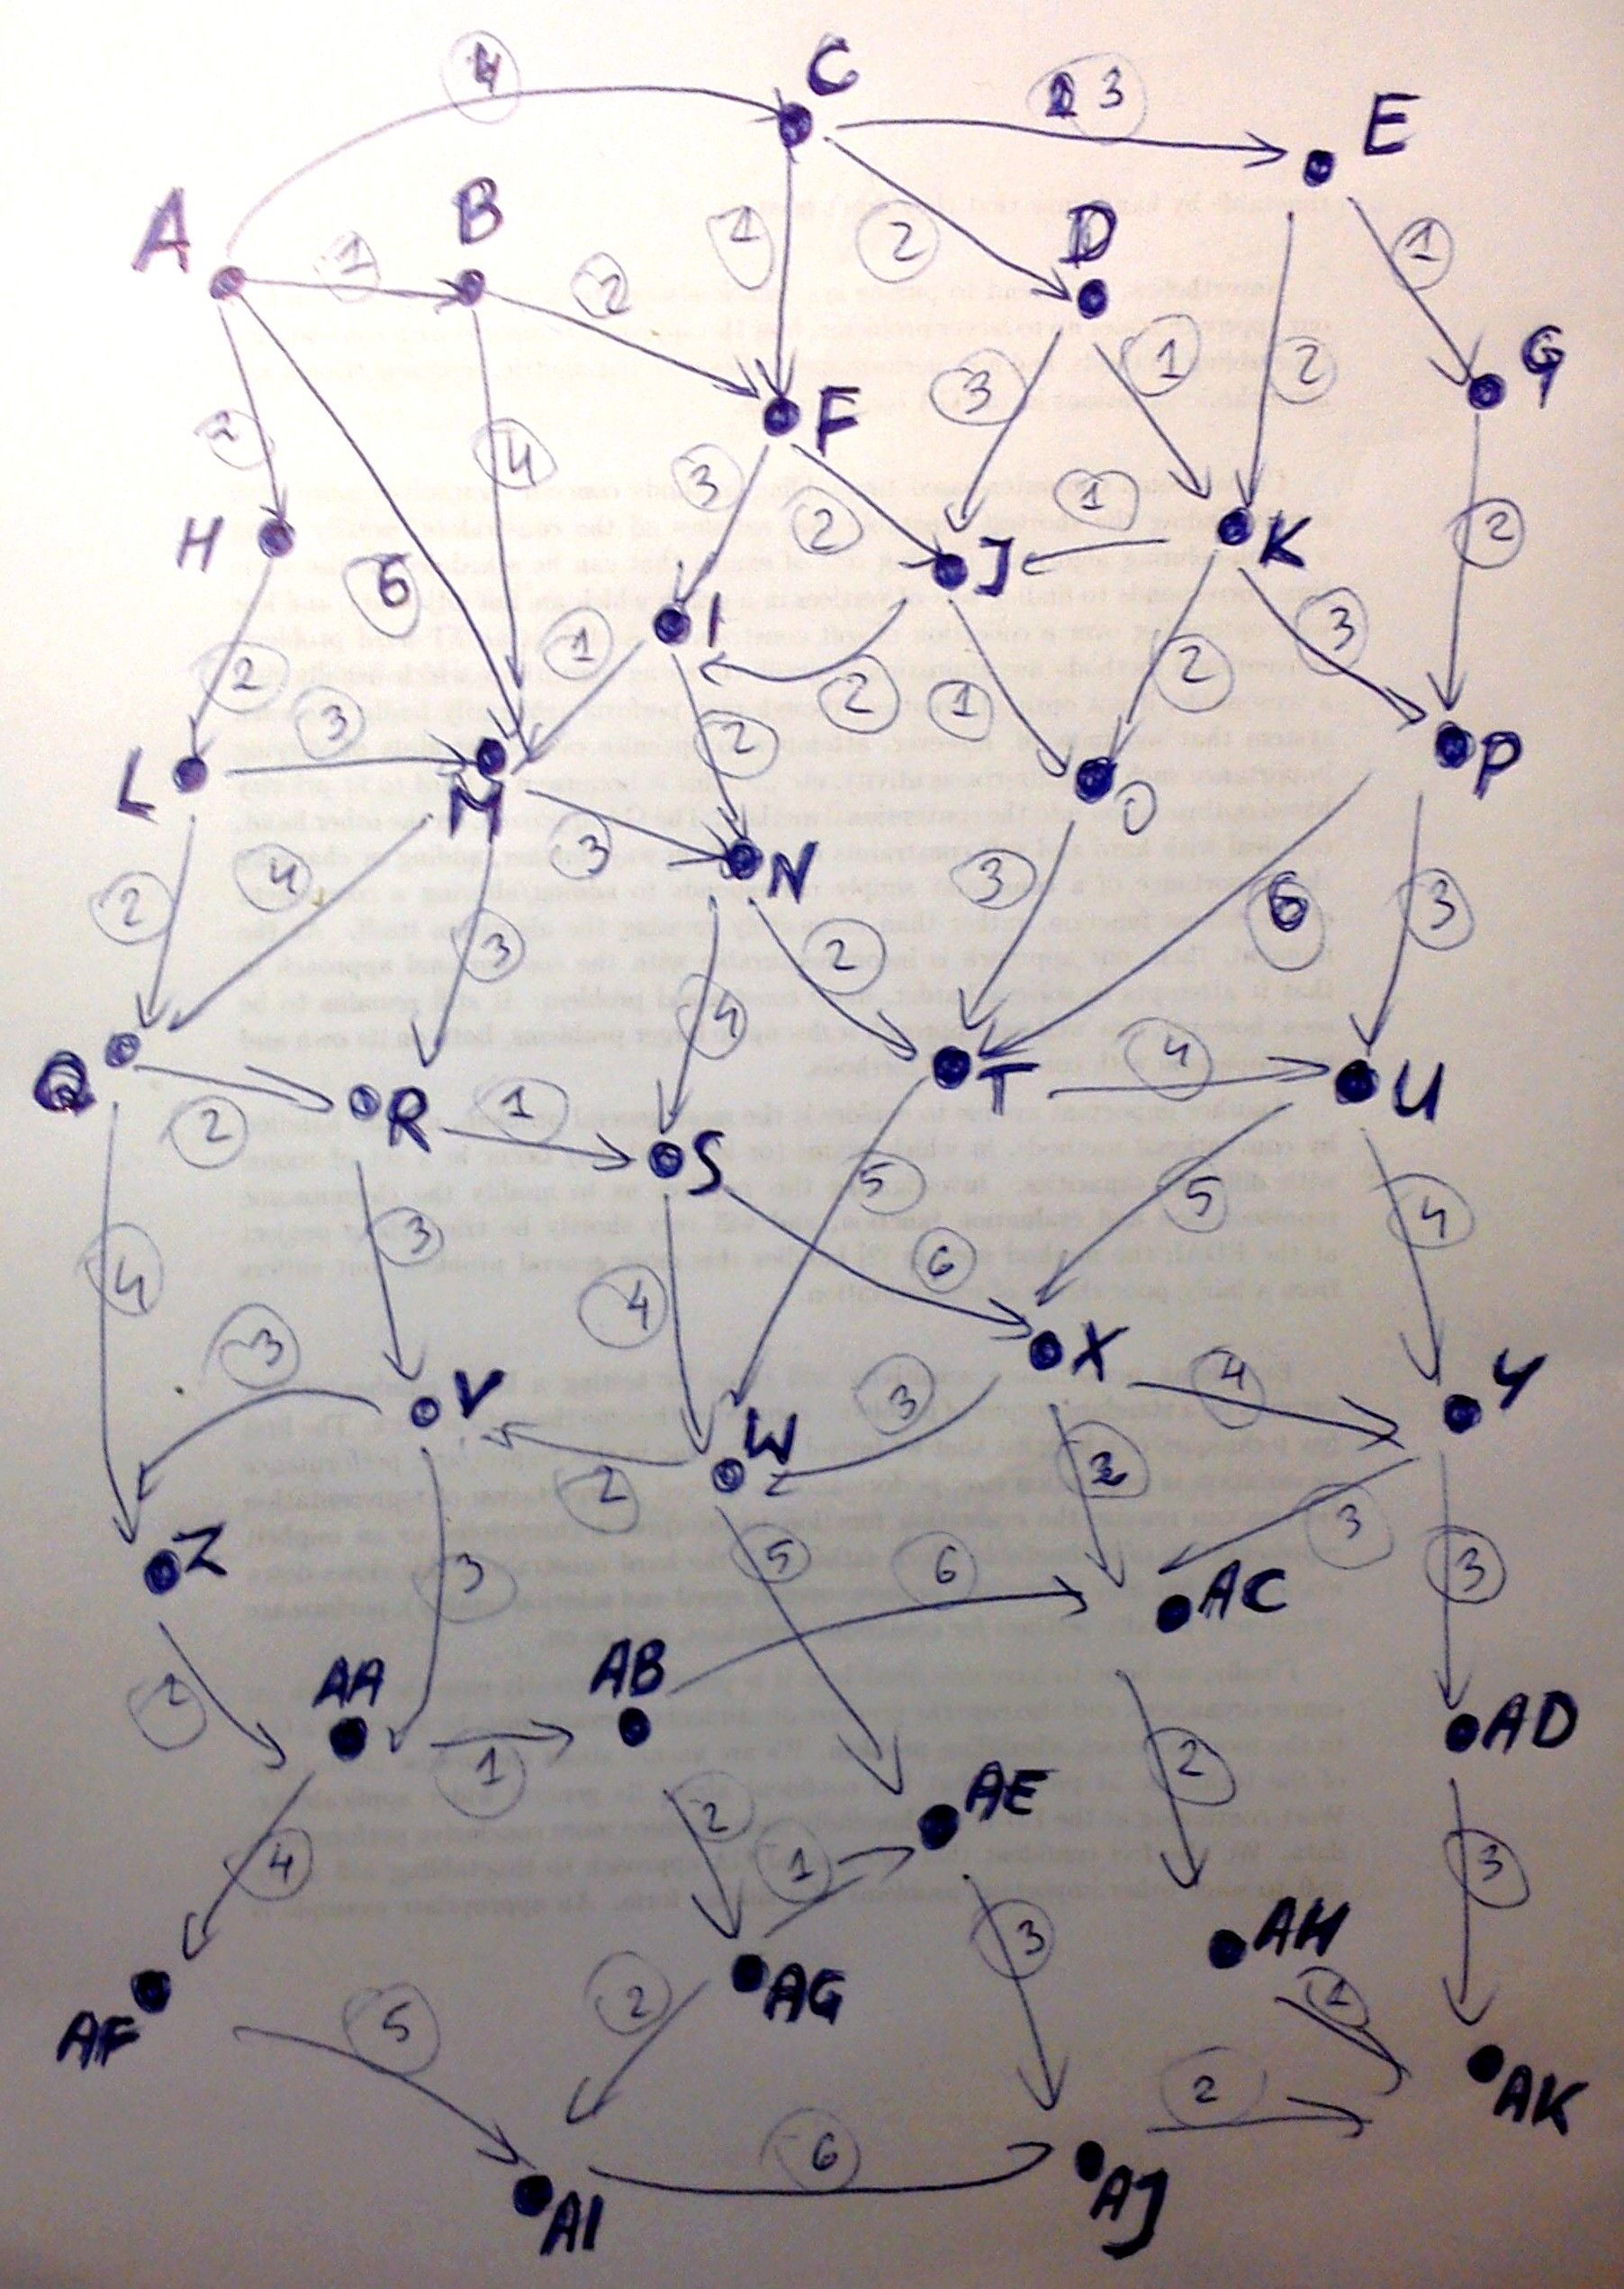
\includegraphics[width=.55\textwidth]{res/testcase3}
	\caption{Graf przypadku testowego nr 3}
	\label{testcase3}
\end{figure}

Odnalezione rozwiązanie:

\begin{lstlisting}
Distances (X means no path) = [0, 1, 4, 6, 7, 3, 8, 2, 6, 5, 6, 4, 5, 8, 6, 9, 6, 8, 9, 9, 12, 11, 13, 15, 16, 10, 12, 13, 17, 19, 18, 16, 15, 19, 17, 21, 20]
PrevNodes (X means initialNode) = [X, 0, 0, 2, 2, 1, 4, 0, 5, 5, 9, 7, 1, 8, 9, 10, 11, 12, 17, 14, 15, 17, 18, 18, 20, 16, 25, 26, 23, 24, 22, 26, 27, 28, 32, 30, 33] 
\end{lstlisting}

Liczby w rozwiązaniu odpowiadają kolejnym oznaczeniom literowym na rysunku \ref{testcase3}.


%%%%%%%%%%%%%%%%%%%%%%%%%%%%%%%%%%%%%%%%%%%%%%%%%%%%%%%%%%%%%%%%%%%%%%%%%%



\clearpage
\addcontentsline{toc}{section}{Literatura}
\begin{thebibliography}{9}
\bibitem{gg} Grama, Gupta, ,,Introduction to parallel computing'', p. 10.2-10.3.

\end{thebibliography}

\end{document}